\chapter{Development}

This chapter describes the architecture, implementation structure, runtime interaction model, simulation rules, UI design, and the iterative process used to deliver the final build.

\section{System Design}

The runtime architecture is split by responsibility rather than by scene object alone. This keeps the battle systems readable and makes it easier to test core behaviour directly.

\begin{figure}[H]
\centering

\includegraphics[width=0.93\textwidth]{architecture-diagram.png}
\caption{High-level runtime architecture for \projectname{}.}
\label{fig:architecture}
\end{figure}

This architecture diagram shows the major runtime modules and the direction of interaction between flow, board, cards, units, and UI. It communicates system responsibilities and runtime coordination at a level that a class-level inheritance diagram would not.

\begin{figure}[H]
\centering

\includegraphics[width=0.93\textwidth]{module-map.png}
\caption{Simplified module dependency and responsibility map.}
\label{fig:module-map}
\end{figure}

The module map complements the architecture view. The architecture diagram explains \textit{what} subsystems exist and how they interact; the module map explains \textit{where} those responsibilities live in the codebase. Table \ref{tab:runtime-components} extends those two figures with the final component inventory.

\begin{table}[H]
\centering
\small
\begin{tabular}{llll}
\toprule
\wcell{2.2cm}{\textbf{Area}} & \wcell{3.7cm}{\textbf{Key classes}} & \wcell{4.8cm}{\textbf{Responsibility}} & \wcell{1.8cm}{\textbf{Origin}} \\
\midrule
\wcell{2.2cm}{Core flow} & \wcell{3.7cm}{`GameRoot`, `GameFlowController`, `GameFlowState`, `TurnManager`} & \wcell{4.8cm}{Scene bootstrap, title-battle-result flow, battle session start, turn state, and win/loss resolution} & \wcell{1.8cm}{Group-authored} \\
\wcell{2.2cm}{Cards} & \wcell{3.7cm}{`CardData`, `DeckManager`, `CardResolver`} & \wcell{4.8cm}{Card definitions, deck lifecycle, draw/discard handling, and explicit effect resolution} & \wcell{1.8cm}{Group-authored} \\
\wcell{2.2cm}{Grid} & \wcell{3.7cm}{`GridManager`, `TileView`} & \wcell{4.8cm}{Board generation, occupancy, movement, range queries, and highlight state} & \wcell{1.8cm}{Group-authored} \\
\wcell{2.2cm}{Units} & \wcell{3.7cm}{`UnitController`, `EnemyAI`} & \wcell{4.8cm}{Shared unit state, damage/heal/guard behaviour, and deterministic enemy targeting and movement} & \wcell{1.8cm}{Group-authored} \\
\wcell{2.2cm}{Runtime HUD} & \wcell{3.7cm}{`BattleUI`, `BattleHudSnapshot`, `CardButtonView`, `UnitHealthBarView`} & \wcell{4.8cm}{Battle-state presentation, runtime card views, prompts, disabled-card feedback, and world-space health bars} & \wcell{1.8cm}{Group-authored} \\
\wcell{2.2cm}{Presentation} & \wcell{3.7cm}{`UnitVisualShell`, `WorldThemeResources`, `UiThemeResources`} & \wcell{4.8cm}{Board dressing, colour palette, unit silhouettes, and themed UI resource binding} & \wcell{1.8cm}{Local presentation over open-licensed UI assets} \\
\bottomrule
\end{tabular}
\caption{Main runtime components used by the delivered system.}
\label{tab:runtime-components}
\end{table}

The most important architectural boundary is the separation between battle rules and presentation. `TurnManager` owns turn progression, card-play budget, enemy phase execution, and battle-end state. `DeckManager` owns the draw pile, hand, and discard pile. `CardResolver` resolves card effects explicitly through readable branches instead of a large effect hierarchy. `GridManager` and `TileView` maintain board occupancy and targeting support. Together these classes form the deterministic gameplay core.

\section{Implementation Strategy and Iteration Process}

The project was developed through short, evidence-driven iterations rather than as a strict once-through sequence. A design baseline existed early, but the team repeatedly returned to requirements, UI layout, and test scope whenever a playable slice exposed a visible weakness. This working style aligns more closely with agile principles of frequent working software and responsiveness to change than with a rigid waterfall handoff model \cite{agileManifesto2001,royce1970}.

The repository history makes those iterations visible. Instead of one large implementation drop, the worktree shows a sequence of focused increments: repository and baseline setup, prototype stabilisation, validation freeze, front-end flow completion, visual theming, and final HUD repair. Table \ref{tab:iteration-history} summarises the most representative slices.

\begin{table}[H]
\centering
\small
\begin{tabular}{llll}
\toprule
\wcell{2.3cm}{\textbf{Window}} & \wcell{3.2cm}{\textbf{Representative commits}} & \wcell{3.8cm}{\textbf{Focus}} & \wcell{2.7cm}{\textbf{Outcome}} \\
\midrule
\wcell{2.3cm}{01/04--02/04} & \wcell{3.2cm}{\code{22b36f4}, \code{b045777}, \code{814c972}, \code{f2ac529}} & \wcell{3.8cm}{Repository curation, clean baseline, battle-end correction, first regression protection} & \wcell{2.7cm}{A stable prototype base with an early correctness fix} \\
\wcell{2.3cm}{02/04--03/04} & \wcell{3.2cm}{\code{968d396}, \code{7438df9}, \code{2d6a444}, \code{e407e63}} & \wcell{3.8cm}{Architecture alignment, screenshots, diagrams, and prototype evidence} & \wcell{2.7cm}{A reportable prototype with aligned technical artifacts} \\
\wcell{2.3cm}{17/04} & \wcell{3.2cm}{\code{c78434f}} & \wcell{3.8cm}{Validation freeze and archived rerun evidence} & \wcell{2.7cm}{A named baseline for execution and coverage evidence} \\
\wcell{2.3cm}{23/04} & \wcell{3.2cm}{\code{b8c1ab3}} & \wcell{3.8cm}{Session flow shell, gameplay stability, and stronger automated coverage} & \wcell{2.7cm}{A complete title-to-result session loop} \\
\wcell{2.3cm}{23/04--24/04} & \wcell{3.2cm}{\code{c4fa026}, \code{572acb2}} & \wcell{3.8cm}{UI theming, board dressing, and unit presentation} & \wcell{2.7cm}{A clearer visual identity for the tactical slice} \\
\wcell{2.3cm}{24/04} & \wcell{3.2cm}{\code{98753ae}} & \wcell{3.8cm}{HUD readability closure and layout repair} & \wcell{2.7cm}{The most visible UX defects were closed} \\
\wcell{2.3cm}{24/04} & \wcell{3.2cm}{\code{df9ea5a}} & \wcell{3.8cm}{Final report package preparation} & \wcell{2.7cm}{The final-report source tree and appendix scaffolding were assembled} \\
\bottomrule
\end{tabular}
\caption{Representative iterations visible in the repository history.}
\label{tab:iteration-history}
\end{table}

This iterative process mattered because the product was not improved mainly by widening scope. Instead, each iteration targeted one of three questions:

\begin{itemize}
    \item what must be built next to make the current battle slice more complete;
    \item what defect currently blocks understanding, stability, or submission credibility;
    \item what evidence is needed to prove that the change actually holds.
\end{itemize}

That is why flow, HUD readability, and validation work kept rising above more attractive content additions. The backlog was reprioritised by playable evidence, not only by original intention.

\section{Prototype and UI Structure}

The following figures illustrate the information structure and the runtime composition of the playable scene.

\begin{figure}[H]
\centering
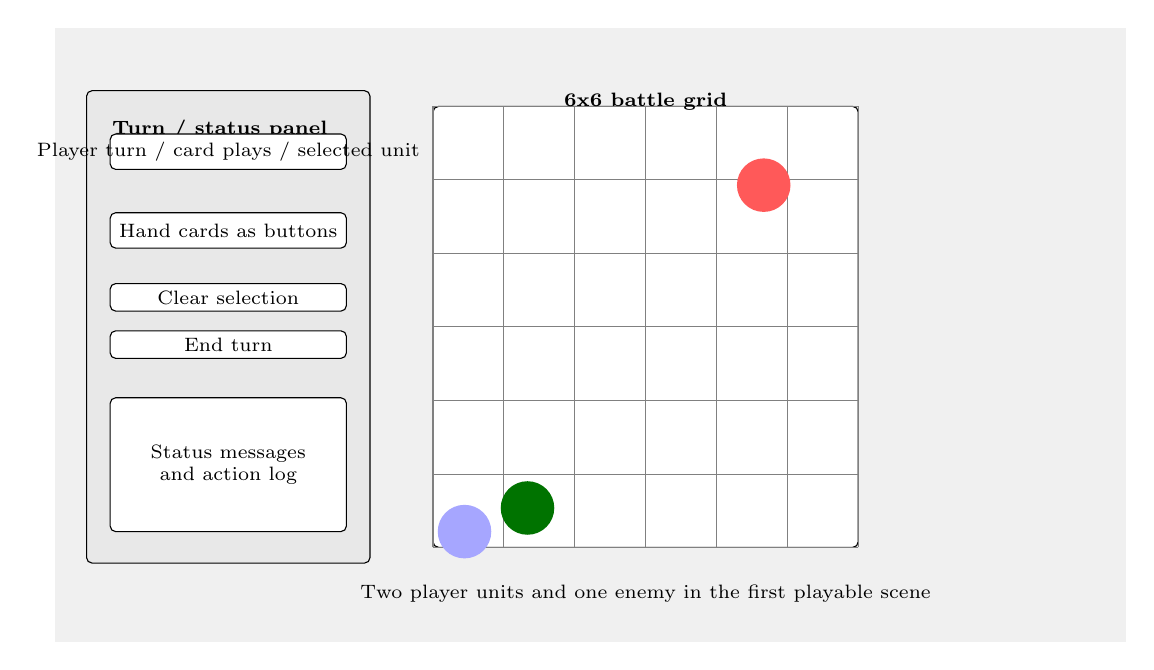
\begin{tikzpicture}[
    x=1cm,
    y=1cm,
    font=\scriptsize,
    panel/.style={draw, rounded corners=2pt, fill=gray!8},
    note/.style={draw, rounded corners=2pt, fill=white, align=center}
]
\fill[gray!12] (0,0) rectangle (13.6,7.8);

\draw[panel, fill=gray!18] (0.4,1.0) rectangle (4.0,7.0);
\node[anchor=north west] at (0.6,6.75) {\textbf{Turn / status panel}};
\draw[note] (0.7,6.0) rectangle (3.7,6.45);
\node at (2.2,6.22) {Player turn / card plays / selected unit};
\draw[note] (0.7,5.0) rectangle (3.7,5.45);
\node at (2.2,5.22) {Hand cards as buttons};
\draw[note] (0.7,4.2) rectangle (3.7,4.55);
\node at (2.2,4.37) {Clear selection};
\draw[note] (0.7,3.6) rectangle (3.7,3.95);
\node at (2.2,3.77) {End turn};
\draw[note] (0.7,1.4) rectangle (3.7,3.1);
\node[text width=2.5cm, align=center] at (2.2,2.25) {Status messages\\and action log};

\draw[panel, fill=white] (4.8,1.2) rectangle (10.2,6.8);
\foreach \x in {4.8,5.7,6.6,7.5,8.4,9.3,10.2} {
    \draw[gray] (\x,1.2) -- (\x,6.8);
}
\foreach \y in {1.2,2.13,3.07,4.0,4.93,5.87,6.8} {
    \draw[gray] (4.8,\y) -- (10.2,\y);
}
\node[anchor=north] at (7.5,7.1) {\textbf{6x6 battle grid}};
\fill[blue!35] (5.2,1.4) circle (0.34);
\fill[green!45!black] (6.0,1.7) circle (0.34);
\fill[red!65] (9.0,5.8) circle (0.34);
\node[anchor=north] at (7.5,0.85) {Two player units and one enemy in the first playable scene};
\end{tikzpicture}

\caption{Low-fidelity wireframe showing the intended information zones.}
\label{fig:retrospective-wireframe}
\end{figure}

\begin{figure}[H]
\centering

\includegraphics[width=0.88\textwidth]{battle-scene-ui.png}
\caption{Battle scene with UI, hand, and 6x6 board.}
\label{fig:prototype-evidence}
\end{figure}

\begin{figure}[H]
\centering

\includegraphics[width=0.88\textwidth]{card-hand-closeup.png}
\caption{Runtime card hand and top-bar state.}
\label{fig:prototype-cards}
\end{figure}

\begin{figure}[H]
\centering

\includegraphics[width=0.88\textwidth]{board-scene-overview.png}
\caption{Board-only view of the playable battle scene.}
\label{fig:prototype-board}
\end{figure}

The wireframe shows the intended information architecture: prompt information, a central board, and a persistent hand zone. The runtime screenshots show how that structure appears in the delivered build.

\section{Reserved Updated Screenshot Set}

The figures above preserve the earlier runtime evidence already referenced by the report. To support a clearer final comparison, the following reserved slots mark where refreshed captures from the latest build should be inserted. These newer captures are intended to sit alongside the earlier figures rather than silently replacing them.

\begin{figure}[H]
\centering
\placeholdergraphic{5.2cm}{Expected replacement: updated main-menu capture showing the branded title overlay, summary panel, and call-to-action button. Suggested file name: `title-screen-final.png`.}
\caption{Reserved slot for the updated main-menu screen, to be compared with the earlier information architecture in Figure \ref{fig:retrospective-wireframe}.}
\label{fig:updated-title-placeholder}
\end{figure}

\begin{figure}[H]
\centering
\placeholdergraphic{5.2cm}{Expected replacement: updated battle-overview capture showing the final board dressing, HUD, and unit presentation. Suggested file name: `battle-screen-final.png`.}
\caption{Reserved slot for the updated battle view, to be compared with the earlier runtime battle screenshot in Figure \ref{fig:prototype-evidence}.}
\label{fig:updated-battle-placeholder}
\end{figure}

\begin{figure}[H]
\centering
\placeholdergraphic{5.2cm}{Expected replacement: updated card-interface capture showing the hand dock, prompt bar, and action feedback. Suggested file name: `card-interface-final.png`.}
\caption{Reserved slot for the updated card-interface capture, to be compared with the earlier hand-and-top-bar view in Figure \ref{fig:prototype-cards}.}
\label{fig:updated-card-ui-placeholder}
\end{figure}

\begin{figure}[H]
\centering
\placeholdergraphic{5.2cm}{Expected replacement: representative close-up of a final card face, including icon, title, cost/action hint, and descriptive text. Suggested file name: `card-face-final.png`.}
\caption{Reserved slot for a close-up of the final card-face design.}
\label{fig:updated-card-face-placeholder}
\end{figure}

\begin{figure}[H]
\centering
\placeholdergraphic{5.2cm}{Expected replacement: victory result screen showing final end-state presentation and replay/menu actions. Suggested file name: `result-victory-final.png`.}
\caption{Reserved slot for the victory result screen, documenting the completed positive end-state flow.}
\label{fig:updated-victory-placeholder}
\end{figure}

\begin{figure}[H]
\centering
\placeholdergraphic{5.2cm}{Expected replacement: defeat result screen showing final end-state presentation and replay/menu actions. Suggested file name: `result-defeat-final.png`.}
\caption{Reserved slot for the defeat result screen, documenting the alternate end-state flow.}
\label{fig:updated-defeat-placeholder}
\end{figure}

\section{Code Structure}

The project is built around a small set of scene-bound `MonoBehaviour` scripts plus a few light model or helper types, so folder and responsibility views communicate the runtime better than a large inheritance tree would.

\begin{Verbatim}[fontsize=\small]
Assets/Scripts
|-- Cards
|   |-- CardData.cs
|   |-- CardResolver.cs
|   `-- DeckManager.cs
|-- Common
|   `-- GameEnums.cs
|-- Core
|   |-- GameFlowController.cs
|   |-- GameFlowState.cs
|   |-- GameRoot.cs
|   `-- TurnManager.cs
|-- Grid
|   |-- GridManager.cs
|   `-- TileView.cs
|-- Presentation
|   |-- UnitVisualShell.cs
|   `-- WorldThemeResources.cs
|-- UI
|   |-- BattleHudModels.cs
|   |-- BattleUI.cs
|   |-- CardButtonView.cs
|   |-- UiThemeResources.cs
|   `-- UnitHealthBarView.cs
`-- Units
    |-- EnemyAI.cs
    `-- UnitController.cs
\end{Verbatim}

The implementation stays focused on a single battle slice. The battlefield, deck flow, and enemy response remain intentionally compact so that interaction clarity and system stability take priority over content breadth.

\section{Unity Engine-Level Implementation Details}

\begin{table}[H]
\centering
\small
\begin{tabular}{lll}
\toprule
\wcell{3.2cm}{\textbf{Concern}} & \wcell{4.1cm}{\textbf{Actual implementation in the final build}} & \wcell{4.2cm}{\textbf{Reason this choice was kept}} \\
\midrule
\wcell{3.2cm}{Runtime UI root} & \wcell{4.1cm}{`GameFlowController` creates a `ScreenSpaceOverlay` `Canvas` with `CanvasScaler`, `GraphicRaycaster`, and `InputSystemUIInputModule`.} & \wcell{4.2cm}{Keeps title, battle, and result flow in one scene and simplifies testing of flow state.} \\
\wcell{3.2cm}{Board interaction path} & \wcell{4.1cm}{`BattleUI` reads `Mouse.current`, checks `EventSystem.current.IsPointerOverGameObject()`, and then uses `Physics.Raycast` for board clicks.} & \wcell{4.2cm}{Directly links card selection to tile and unit selection without building a heavier custom input layer.} \\
\wcell{3.2cm}{Tile interaction surface} & \wcell{4.1cm}{`GridManager` creates tiles as `PrimitiveType.Cube`, which provides colliders for click and occupancy interaction.} & \wcell{4.2cm}{Simple primitive generation makes the board easy to build, raycast, and validate.} \\
\wcell{3.2cm}{Presentation props} & \wcell{4.1cm}{World dressing uses generated primitives with colliders removed or disabled through the presentation helper path.} & \wcell{4.2cm}{Prevents decorative props from blocking tactical interaction while preserving scene dressing.} \\
\wcell{3.2cm}{UI-state separation} & \wcell{4.1cm}{`BattleUI` builds `BattleHudSnapshot` and card-view models instead of reading scattered fields ad hoc.} & \wcell{4.2cm}{Improves testability and reduces the risk of late HUD regressions.} \\
\wcell{3.2cm}{Debug entry path} & \wcell{4.1cm}{Direct-battle debug mode is routed through the shared flow bootstrap instead of bypassing the real HUD.} & \wcell{4.2cm}{Ensures smoke and automated checks exercise the same runtime tree the player actually sees.} \\
\bottomrule
\end{tabular}
\caption{Unity engine-level implementation details.}
\label{tab:unity-implementation-details}
\end{table}

\section{Simulation Design}

The delivered game simulates one compact tactical encounter on a 6x6 grid. Two player-controlled units occupy the board at battle start and fight one or more enemies under a turn-based loop. The simulation is deliberately deterministic: there are no random enemy tactics, no procedural map changes, and no branching objectives. This makes the battle state easier to understand for players and easier to validate for the development team.

At the start of each player turn, `TurnManager` refreshes the action budget and asks `DeckManager` to discard the previous hand and draw a new one. In the delivered build, the player draws three cards per turn and may spend two actions (`maxCardPlaysPerTurn = 2`). This keeps the turn short enough to remain readable while still allowing combinations such as move plus attack or defend plus reposition.

The fallback starter deck contains nine runtime cards:

\begin{itemize}
    \item three `Move` cards;
    \item one `Dash`;
    \item one `Strike`;
    \item one `Long Strike`;
    \item one `Guard`;
    \item one `Push`;
    \item one `Recover`.
\end{itemize}

`CardResolver` keeps the effect logic explicit. Movement and dash actions resolve against tiles, strike and push actions resolve against enemy units, and guard or recover resolve against the acting unit. Enemy behaviour remains deterministic: `EnemyAI` selects the nearest alive player unit by Manhattan distance and either attacks when adjacent or steps toward the target.

\section{UI Design}

The front-end flow is assembled at runtime by `GameFlowController`. It creates the runtime canvas, builds title, battle, and result panels, and keeps them inside the same main scene. The title panel includes the game brand, a short summary, a feature strip, and a clear call to action. The result panel exposes the battle outcome plus replay and menu actions.

During battle, `BattleUI` builds a three-zone runtime HUD:

\begin{itemize}
    \item a top bar for turn state, remaining energy, selection state, prompts, and action buttons;
    \item a left panel for unit summary, status, and the battle log;
    \item a bottom panel for the active hand of cards.
\end{itemize}

The runtime HUD does not pull ad hoc strings directly from scattered private state. Instead, it builds a `BattleHudSnapshot` containing turn labels, prompt text, selected-unit information, card states, and unit summaries. `CardButtonView` uses this snapshot to render card title, description, use hints, and disabled reasons directly in the hand. `UnitHealthBarView` projects health state back into world space so HP can be read from the board rather than only from the log.

Visual theming is added without replacing the project's own runtime structure. The interface uses themed UI resources for banners, panels, buttons, and symbols, while the board, props, and unit silhouettes remain driven by the project's own presentation code. The result is still a compact demo, but it now looks intentional rather than merely assembled.
